\documentclass[11pt,a4paper]{article}

\usepackage[T1]{fontenc}
\usepackage[utf8]{inputenc}
\usepackage{lmodern}
\usepackage[margin=18mm]{geometry}
\usepackage{microtype}
\usepackage{booktabs}
\usepackage{tabularx}
\usepackage{xcolor}
\usepackage{hyperref}
\usepackage{enumitem}
\usepackage{caption}
\usepackage{tikz}
\usepackage{pgfplots}
\usepackage{array}
\usepackage{colortbl}

\pgfplotsset{compat=1.18}
\usetikzlibrary{positioning}

\definecolor{muted}{HTML}{5F5B55}
\definecolor{blue}{HTML}{1D4E89}
\definecolor{amber}{HTML}{8A5A12}
\definecolor{hlrow}{HTML}{EEF3F9}
\definecolor{capc}{HTML}{D9D3C7}
\definecolor{restc}{HTML}{8AA4C4}
\definecolor{boxbg}{HTML}{F6F3EC}

\hypersetup{colorlinks=true,linkcolor=blue,urlcolor=blue,
  pdftitle={Sample-based index evaluation: reviewer note}}

\newcolumntype{L}{>{\raggedright\arraybackslash}X}

\pagestyle{plain}
\setlength{\parskip}{0.32em}
\setlength{\parindent}{0pt}
\setlist[itemize]{leftmargin=1.3em,itemsep=0.12em,topsep=0.2em}
\setlist[enumerate]{leftmargin=1.4em,itemsep=0.15em,topsep=0.2em}
\captionsetup{font=small,skip=4pt}

\title{\vspace{-12mm}Sample-based index evaluation}
\author{Reviewer note (COL868)}
\date{PostgreSQL 14, TPC-DS SF=1, 99 queries, 33 configurations, 5\% samples, one seed.\\
5--6 October 2026.}

\begin{document}
\maketitle
\vspace{-10mm}

\section{Question}

Optimizer cost is an unreliable ranking of indexes (Wu et al., SIGMOD 2025). Timing every candidate on the full database is too expensive. \textbf{Does a 5\% sample recover the same execution-time ranking?} Closest prior work, SQL:Trek (PVLDB 2025), uses one 5\% Bernoulli recipe and does not report agreement with a full-database ranking of the same configurations.

\textbf{Supported here:} on this SF=1 run, cheap random samples pick a configuration within 1.4\% of the full-database winner, at 25--90$\times$ lower eval cost, and rank no worse than the full database ranks itself (tau $\approx$ 0.45). Join-aware sampling and copying full statistics did not help.

\textbf{Not supported:} that this holds at 100\,GB, on SQL Server, or that any sampler is strictly better than another.

\section{What was run}

{\small
\begin{tabularx}{\textwidth}{@{}p{0.28\textwidth}p{0.36\textwidth}L@{}}
\toprule
Assignment & This run & Why \\
\midrule
SQL Server, 100\,GB TPC-DS & PostgreSQL 14, SF=1 ($\sim$1\,GB, in memory) & SF=10 queries ran for hours on a 16\,GB laptop. \\
Samples at 1\%, 5\%, 10\% & 5\%, one seed & Time. \\
Best index per query & Whole-workload configuration (1--8 indexes) & Per-query winners flipped between identical full-DB runs. \\
Cost and time & Ranked by measured time (A). Score B = build + time. & The question is execution time. \\
Random / stratified / stats / workload-aware & Bernoulli, page, universe, FK, stratified; stats copy on two. No workload-aware. & \\
\bottomrule
\end{tabularx}
}

\section{How it is implemented}

\begin{center}
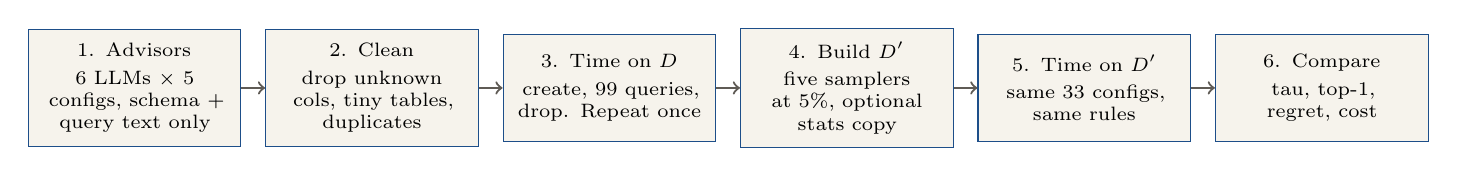
\begin{tikzpicture}[
  box/.style={draw=blue, fill=boxbg, align=center, font=\scriptsize, inner sep=5pt, text width=2.35cm, minimum height=1.35cm},
  arr/.style={->, thick, muted}
]
\node[box] (a) {1. Advisors\\[2pt]6 LLMs $\times$ 5 configs, schema + query text only};
\node[box, right=3mm of a] (b) {2. Clean\\[2pt]drop unknown cols, tiny tables, duplicates};
\node[box, right=3mm of b] (c) {3. Time on $D$\\[2pt]create, 99 queries, drop. Repeat once};
\node[box, right=3mm of c] (d) {4. Build $D'$\\[2pt]five samplers at 5\%, optional stats copy};
\node[box, right=3mm of d] (e) {5. Time on $D'$\\[2pt]same 33 configs, same rules};
\node[box, right=3mm of e] (f) {6. Compare\\[2pt]tau, top-1, regret, cost};
\draw[arr] (a) -- (b); \draw[arr] (b) -- (c); \draw[arr] (c) -- (d); \draw[arr] (d) -- (e); \draw[arr] (e) -- (f);
\end{tikzpicture}
\end{center}

\textbf{Candidates.} Isolated agents see schema, existing indexes, and the 99 query texts. They do not see data or previous timings. One Gemini run opened earlier result files and was thrown out. After cleaning: 33 configurations. Baselines: no extra index, HypoPG greedy top-5 and top-8 (ranked by estimated cost, then timed for real).

\textbf{One configuration at a time.} \texttt{CREATE INDEX} (timed), run all 99 queries, \texttt{DROP}. Leftover indexes from a killed run are dropped first so they cannot leak into the next config.

\textbf{Timing a query.} Autovacuum off. \texttt{ANALYZE} once per database, then frozen (a stats fingerprint is stored with every result row). Discard one warm-up. Then two timed runs if that warm-up was $\le$ 2\,s, else one. Median. Cap 20\,s, counted as 20\,s on both $D$ and $D'$.

\textbf{Scores.} A = sum of 99 query times (primary). B = index-build time + A. Lower is better. A timeout or error is 20\,s.

\textbf{Comparison.} Kendall tau-b with a 95\% bootstrap over the 33 configs. Top-1 is exact. Regret is $D$'s time of $D'$'s pick divided by $D$'s best (1.014 = 1.4\% slower). Cost reduction is (build + workload over all configs on $D$) / (the same on $D'$).

\subsection{How a sample is built}

Target size per table $T$ follows SQL:Trek: keep
\[
k_T = \min\bigl(\max(p\,n_T,\; 20{,}000),\; 10^6\cdot(p/0.05),\; n_T\bigr)
\]
at $p=0.05$. Small tables are oversampled; huge tables are capped.

{\small
\begin{tabularx}{\textwidth}{@{}p{0.22\textwidth}L@{}}
\toprule
Sampler & Rule \\
\midrule
Bernoulli & Each row of each table kept independently with probability $k_T/n_T$. Shrinks facts and dimensions ($\sim$230\,MB). \\
Page & Same size, \texttt{TABLESAMPLE SYSTEM} (whole disk pages). Cheapest to build. \\
Universe (item) & Keep a fact row iff $\mathrm{hash}(\texttt{item\_sk})\bmod 10^4 < 100p$. Same hash in every fact that joins on item. Dimension tables kept in full ($\sim$530\,MB). \\
FK closure & Bernoulli on the three sales facts. Keep matching returns. Thin inventory among sampled items. Dimensions in full. \\
Stratified & On sales, keep at least 5 rows per sold-date, then Bernoulli. Other facts as Bernoulli. Dimensions in full. \\
Stats transplant & Same physical rows. Copy full-DB column statistics and set \texttt{reltuples}/\texttt{relpages} to the full values. Do not \texttt{ANALYZE} after. Indexes on the sample stay small. \\
\bottomrule
\end{tabularx}
}

Independent 5\% on two join partners keeps about $0.25\%$ of matches. That is why universe and FK exist. They pay for it by leaving dimensions whole, so they stay large.

\section{Results}

No extra index: \textbf{190.7\,s}. Best (Grok, small dimension filters): \textbf{172.9\,s}. Spread 17.7\,s.

\begin{figure}[htbp]
\centering

\begin{tikzpicture}
\fill[capc] (0,0) rectangle (8.8*140/190.7,0.55);
\fill[restc] (8.8*140/190.7,0) rectangle (8.8*172.9/190.7,0.55);
\fill[blue] (8.8*172.9/190.7,0) rectangle (8.8,0.55);
\node[font=\small] at (8.8*70/190.7,0.27) {140\,s capped};
\node[font=\small] at (8.8*156.5/190.7,0.27) {33\,s left};
\node[font=\small, white] at (8.8*181.8/190.7,0.27) {18\,s won};
\end{tikzpicture}
\caption{No-index total 190.7\,s. Seven queries hit the 20\,s cap under every configuration, including the best, so 140\,s of every total cannot move. Indexes only rearrange the other $\sim$50\,s.}
\end{figure}

A second full run the next morning: same winner and second place, \textbf{tau 0.45} [0.18, 0.67], every config $\sim$5.3\,s slower. That 0.45 is the noise ceiling.

\begin{figure}[htbp]
\centering
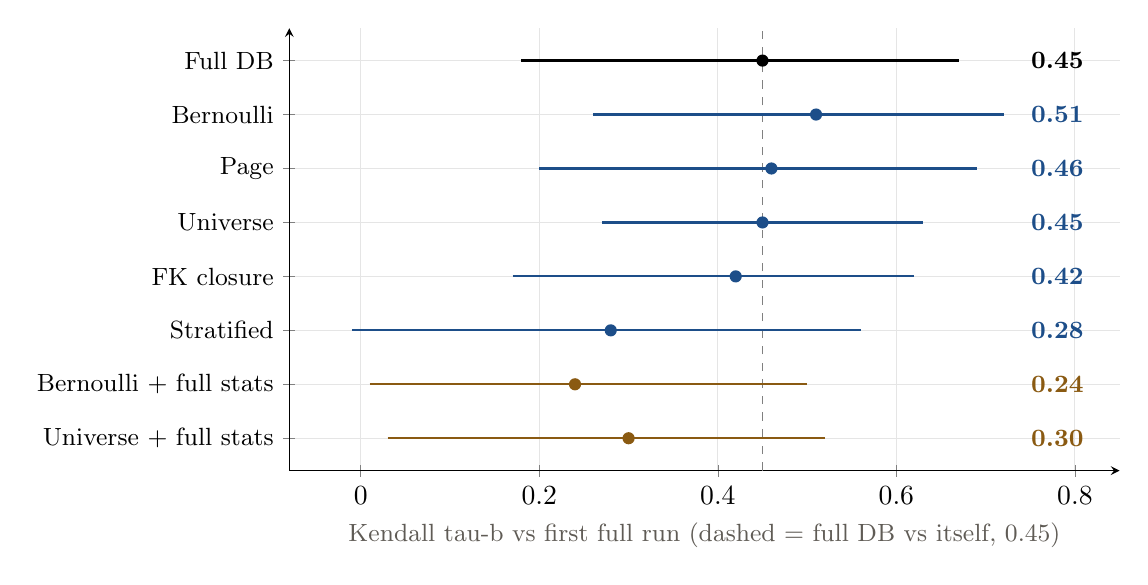
\begin{tikzpicture}
\begin{axis}[
  xmin=-0.08, xmax=0.85, ymin=0.4, ymax=8.6,
  width=\textwidth, height=7.2cm,
  xlabel={Kendall tau-b vs first full run (dashed = full DB vs itself, 0.45)},
  xlabel style={font=\small, color=muted},
  ytick={1,2,3,4,5,6,7,8},
  yticklabels={Universe + full stats, Bernoulli + full stats, Stratified, FK closure, Universe, Page, Bernoulli, Full DB, second run},
  yticklabel style={font=\small, align=right},
  xtick={0,0.2,0.4,0.6,0.8},
  grid=major, major grid style={color=black!10},
  axis lines=left, clip=false,
]
\draw[dashed, black!50] (axis cs:0.45,0.4) -- (axis cs:0.45,8.6);
\draw[black, thick] (axis cs:0.18,8) -- (axis cs:0.67,8);
\fill[black] (axis cs:0.45,8) circle (2.2pt);
\node[font=\small\bfseries, black, anchor=west] at (axis cs:0.74,8) {0.45};
\draw[blue, thick] (axis cs:0.26,7) -- (axis cs:0.72,7);
\fill[blue] (axis cs:0.51,7) circle (2.2pt);
\node[font=\small\bfseries, blue, anchor=west] at (axis cs:0.74,7) {0.51};
\draw[blue, thick] (axis cs:0.20,6) -- (axis cs:0.69,6);
\fill[blue] (axis cs:0.46,6) circle (2.2pt);
\node[font=\small\bfseries, blue, anchor=west] at (axis cs:0.74,6) {0.46};
\draw[blue, thick] (axis cs:0.27,5) -- (axis cs:0.63,5);
\fill[blue] (axis cs:0.45,5) circle (2.2pt);
\node[font=\small\bfseries, blue, anchor=west] at (axis cs:0.74,5) {0.45};
\draw[blue, thick] (axis cs:0.17,4) -- (axis cs:0.62,4);
\fill[blue] (axis cs:0.42,4) circle (2.2pt);
\node[font=\small\bfseries, blue, anchor=west] at (axis cs:0.74,4) {0.42};
\draw[blue, thick] (axis cs:-0.01,3) -- (axis cs:0.56,3);
\fill[blue] (axis cs:0.28,3) circle (2.2pt);
\node[font=\small\bfseries, blue, anchor=west] at (axis cs:0.74,3) {0.28};
\draw[amber, thick] (axis cs:0.01,2) -- (axis cs:0.50,2);
\fill[amber] (axis cs:0.24,2) circle (2.2pt);
\node[font=\small\bfseries, amber, anchor=west] at (axis cs:0.74,2) {0.24};
\draw[amber, thick] (axis cs:0.03,1) -- (axis cs:0.52,1);
\fill[amber] (axis cs:0.30,1) circle (2.2pt);
\node[font=\small\bfseries, amber, anchor=west] at (axis cs:0.74,1) {0.30};
\end{axis}
\end{tikzpicture}
\caption{95\% bootstrap CI over 33 configs. Blue: native 5\%. Brown: same rows, full-DB statistics copied on.}
\end{figure}

{\footnotesize
\begin{tabularx}{\textwidth}{@{}l r l c r c r L@{}}
\toprule
Sample & tau & 95\% CI & Top-1 & Regret & Top-3 & Cheaper & Pick \\
\midrule
Bernoulli & 0.51 & 0.26--0.72 & no & 1.014 & yes & 43$\times$ (25$\times$) & Opus light \\
Page & 0.46 & 0.20--0.69 & no & 1.014 & yes & 90$\times$ (33$\times$) & Opus light \\
Universe & 0.45 & 0.27--0.63 & no & 1.014 & yes & 2.6$\times$ & Opus light \\
FK closure & 0.42 & 0.17--0.62 & no & 1.014 & yes & 3.5$\times$ & Opus light \\
Stratified & 0.28 & $-$0.01--0.56 & yes & 1.000 & yes & 3.4$\times$ & Grok small \\
\rowcolor{hlrow}
Bernoulli, full stats & 0.24 & 0.01--0.50 & no & 1.014 & no & 30$\times$ & Opus light \\
\rowcolor{hlrow}
Universe, full stats & 0.30 & 0.03--0.52 & no & 1.078 & yes & 2.4$\times$ & Composer mixed \\
\bottomrule
\end{tabularx}
}

{\small Cost in parentheses includes building the sample. Grok small is the true best (172.9\,s). Opus light is 175.4\,s (1.4\% slower). Native samples always put those two in the top 2. Score B does not change picks except stratified, which then also misses. Copying full statistics made both rankings worse. Intervals overlap; one seed.}

\begin{figure}[htbp]
\centering
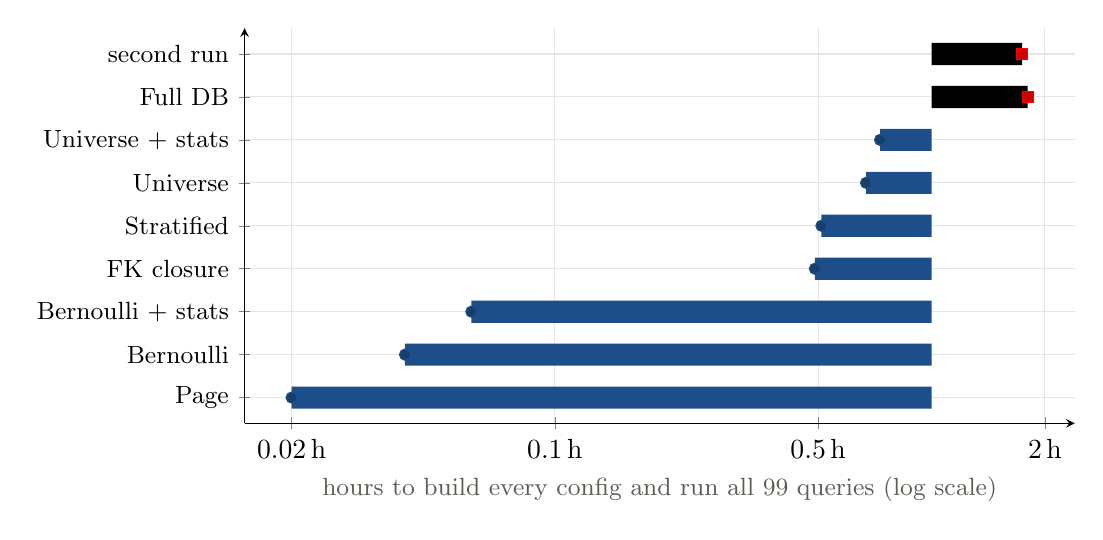
\begin{tikzpicture}
\begin{axis}[
  xmode=log, xmin=0.015, xmax=2.4,
  ymin=0.4, ymax=9.6,
  width=\textwidth, height=6.6cm,
  xlabel={hours to build every config and run all 99 queries (log scale)},
  xlabel style={font=\small, color=muted},
  ytick={1,2,3,4,5,6,7,8,9},
  yticklabels={Page, Bernoulli, Bernoulli + stats, FK closure, Stratified, Universe, Universe + stats, Full DB, second run, Full DB},
  yticklabel style={font=\small, align=right},
  xtick={0.02,0.1,0.5,2},
  xticklabels={0.02\,h, 0.1\,h, 0.5\,h, 2\,h},
  grid=major, major grid style={color=black!10},
  axis lines=left,
]
\addplot+[xbar, fill=blue, draw=none, bar width=8pt] coordinates {
  (0.02,1) (0.04,2) (0.06,3) (0.49,4) (0.51,5) (0.67,6) (0.73,7)
};
\addplot+[xbar, fill=black, draw=none, bar width=8pt] coordinates {
  (1.80,8) (1.74,9)
};
\end{axis}
\end{tikzpicture}
\caption{Join-aware samples keep dimension tables whole, so they only save $\sim$3$\times$. Bernoulli and page shrink every table.}
\end{figure}

\begin{figure}[htbp]
\centering
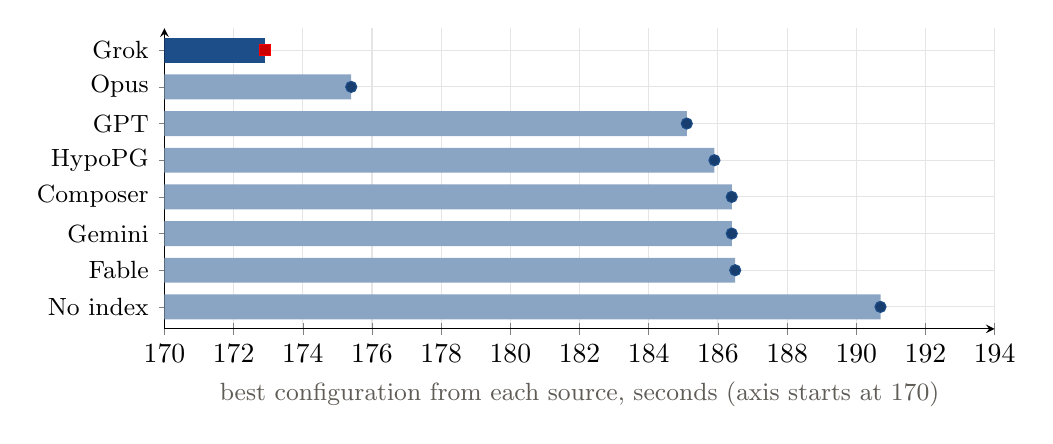
\begin{tikzpicture}
\begin{axis}[
  xmin=170, xmax=194,
  ymin=0.4, ymax=8.6,
  width=\textwidth, height=5.4cm,
  xlabel={best configuration from each source, seconds (axis starts at 170)},
  xlabel style={font=\small, color=muted},
  ytick={1,2,3,4,5,6,7,8},
  yticklabels={No index, Fable, Gemini, Composer, HypoPG, GPT, Opus, Grok},
  yticklabel style={font=\small, align=right},
  grid=major, major grid style={color=black!10},
  axis lines=left,
]
\addplot+[xbar, fill=restc, draw=none, bar width=9pt] coordinates {
  (190.7,1) (186.5,2) (186.4,3) (186.4,4) (185.9,5) (185.1,6) (175.4,7)
};
\addplot+[xbar, fill=blue, draw=none, bar width=9pt] coordinates {(172.9,8)};
\end{axis}
\end{tikzpicture}
\caption{HypoPG's greedy set, ranked by optimizer cost then timed, lands in the middle. Empty is the slowest of the 33. Only Grok and Opus moved the needle much.}
\end{figure}

\begin{figure}[htbp]
\centering
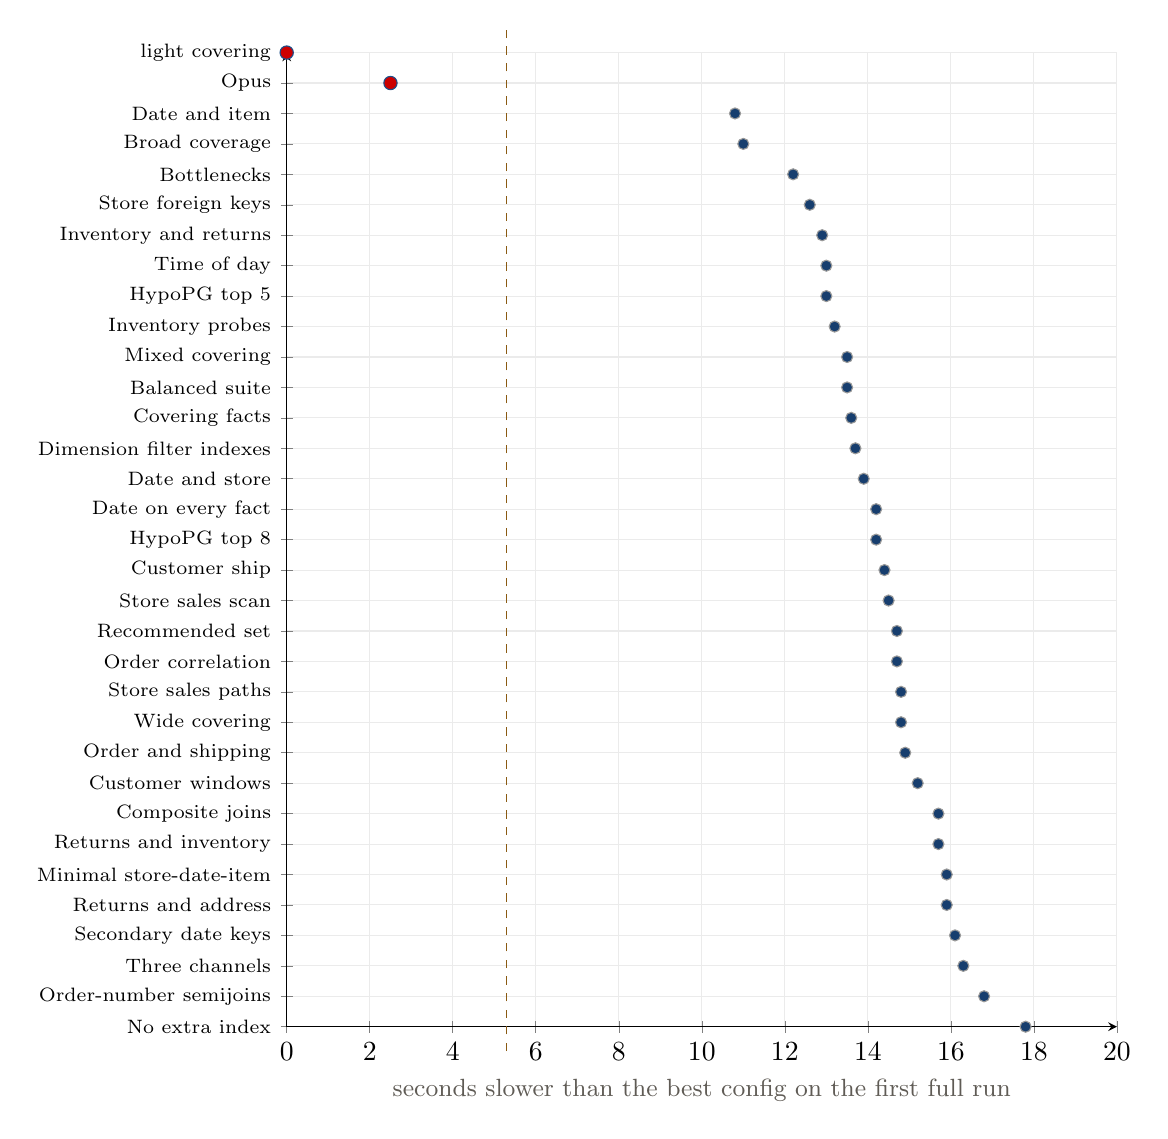
\begin{tikzpicture}
\begin{axis}[
  xmin=0, xmax=20,
  width=\textwidth, height=14.2cm,
  xlabel={seconds slower than the best config on the first full run},
  xlabel style={font=\small, color=muted},
  y=11pt,
  ytick={1,...,33},
  yticklabels={
    No extra index,
    Order-number semijoins,
    Three channels,
    Secondary date keys,
    Returns and address,
    Minimal store-date-item,
    Returns and inventory,
    Composite joins,
    Customer windows,
    Order and shipping,
    Wide covering,
    Store sales paths,
    Order correlation,
    Recommended set,
    Store sales scan,
    Customer ship,
    HypoPG top 8,
    Date on every fact,
    Date and store,
    Dimension filter indexes,
    Covering facts,
    Balanced suite,
    Mixed covering,
    Inventory probes,
    HypoPG top 5,
    Time of day,
    Inventory and returns,
    Store foreign keys,
    Bottlenecks,
    Broad coverage,
    Date and item,
    Opus, light covering,
    Grok, dimension filters
  },
  yticklabel style={font=\scriptsize, align=right},
  grid=major, major grid style={color=black!8},
  axis lines=left, clip=false,
]
\draw[dashed, amber] (axis cs:5.3,0.2) -- (axis cs:5.3,33.8);
\addplot+[only marks, mark=*, mark size=2pt, fill=black!40, draw=black!40] coordinates {
  (17.8,1) (16.8,2) (16.3,3) (16.1,4) (15.9,5) (15.9,6) (15.7,7) (15.7,8)
  (15.2,9) (14.9,10) (14.8,11) (14.8,12) (14.7,13) (14.7,14) (14.5,15)
  (14.4,16) (14.2,17) (14.2,18) (13.9,19) (13.7,20) (13.6,21) (13.5,22)
  (13.5,23) (13.2,24) (13.0,25) (13.0,26) (12.9,27) (12.6,28) (12.2,29)
  (11.0,30) (10.8,31)
};
\addplot+[only marks, mark=*, mark size=2.4pt, fill=blue, draw=blue] coordinates {
  (2.5,32) (0,33)
};
\end{axis}
\end{tikzpicture}
\caption{Dashed line: 5.3\,s median overnight shift. Winner and second are 2.4\,s apart, inside that shift. 31 of 33 configs sit within 4\%. That is why tau against a repeat of the full database is only 0.45.}
\end{figure}

The two winners mainly cut Q6 (20\,s cap $\to$ $\sim$10\,s) and Q14 (7.0 $\to$ $\sim$3.7\,s), both via date-dimension filter indexes. Inferred from per-query times, not an ablation.

{\small
\begin{tabularx}{\textwidth}{@{}p{0.42\textwidth}L@{}}
\toprule
Expectation & Outcome \\
\midrule
Sample finds the execution-time best. & Exact top-1 on 1 of 5 native samples. Others 1.4\% off; true best always in top 3. \\
Join-aware beats random. & No. Same quality, $\sim$3$\times$ cheaper vs 40--90$\times$. \\
Full statistics improve fidelity. & No, on the two samples tried. \\
Samples rank like the full DB. & To within noise (tau 0.42--0.51 vs ceiling 0.45). \\
\bottomrule
\end{tabularx}
}

\section{Caveats}

\begin{itemize}
\item One seed, one rate, $n=33$ near-ties. Sampler differences of 0.05 in tau are inside the CIs.
\item 20\,s cap hides any index that would have helped the seven always-capped queries, including Q6 under no-index.
\item SF=1 is cache-resident. Assignment was 100\,GB SQL Server.
\item Stats transplant copies table stats only; indexes stay small. Negative result is for this implementation.
\item Candidate pool is clustered. Empty is the only clearly bad config.
\item Measurement choices (cap, score A, SF=1) were informed by an earlier noisy per-query pilot, not blind.
\end{itemize}

\section{What to push on}

\begin{enumerate}
\item Is 1.4\% regret a success when best-to-worst is only 9\% and overnight drift is 5.3\,s?
\item Score A or B? They disagree on stratified top-1.
\item Is tau-vs-self 0.45 a fair ceiling from one repeat?
\item Next measurement that would settle the question: SF=10 on a 64--128\,GB machine, two full rankings, then Bernoulli + page at 1/5/10\% plus one join-consistent sampler, extra seed. More SF=1 cells will not.
\end{enumerate}

\end{document}
